\documentclass[12pt]{article}

\usepackage{amssymb,amsmath,makecell,epsfig,amsthm,listings,bm,hyperref}
\newcommand{\dd}{\mathrm{d}}
\newcommand{\imag}{\mathrm{i}}
\newcommand{\e}{\mathrm{e}}

\newcommand{\R}{\mathbb{R}}
\newcommand{\C}{\mathbb{C}}

\begin{document}
	\title{Approximating contour integral solutions of the parabolic wave equation}
	\maketitle
	
	\section{Problem statement}
	
	In \cite{DavePaper}, it was show that there exist families of solutions to the parabolic wave equation
	\[
	2\imag \frac{\partial u(x,y)}{\partial x} + \frac{\partial^2 u(x,y)}{\partial y^2} = 0,\quad (x,y)\in\R^2.
	\]
	These solutions were of the form:
	\begin{equation}\label{eq:can}
	u(x,y) = \int_\gamma \e^{\imag g(t;x,y)}\dd{t},
	\end{equation}
	where $\gamma$ is an unbounded contour in $\C$ and $g(\cdot;x,y)$ is a polynomial with coefficients depending on $x$ and $y$. Given that the integrand of \eqref{eq:can} is entire, it follows by Cauchy's integral theorem that $\gamma$ can be deformed onto any contour with the same (infinite) endpoints in $\C$. For stable numerical evaluation of \eqref{eq:can}, this contour should be chosen to be on, or close to, the path of steepest descent. One cannot expect a brute force quadrature approach to work if this path is not known, as it is very possible that the integrand will grow exponentially along a given contour, even if this integrand is zero at its endpoints.
	
	\section{Outline of code}
	
	\emph{PathFinder} was developed with the intention of evaluating highly oscillatory integrals over a bounded subset of $\R$ using the method of numerical steepest descent. Although \eqref{eq:can} is not highly oscillatory, we were able to use some components of PathFinder to determine a suitable contour $\gamma$, which is sufficiently close to the path of steepest descent.
	
	Currently, for each $(x,y)\in\R^2$ a separate integral \eqref{eq:can} must be evaluated, which means that evaluation on an $N\times N$ grid in $\R^2$ runs in $O(N^2)$ time. To increase convergence in $N$, we use a tensor product of two Chebyshev grids, and approximate $u(x,y)$ using Chebfun2. To gain back some additional CPU time, the code has been written to run in parallel, so for $P$ cores the code runs in $O(N^2/P)$ time.
	
	\section{Sample code}
	
	Before the code can be used, you must ensure that \href{https://github.com/chebfun/chebfun}{Chebfun} and \href{https://github.com/AndrewGibbs/NSDpackage}{PathFinder} are added to the Matlab search path (including all subfolders).
	
	Once all of the necessary directories have been added, we can define the key components of our integral \eqref{eq:can}. These are the endpoints of the contour $\gamma$ and the coefficients of the polynomial $g$, which in this example are:
	\[
	\texttt{aValley = exp(9i*pi/10); 	bValley = exp(1i*pi/10);}
	\]
	\[
	\texttt{	Pcoeffs = @(X,Y) [2/5 -X/2 0 -Y 0 0];}
	\]
	Notice that the polynomial coefficients vector \texttt{Pcoeffs} is defined as an anonymous function, with dependency on $X$ and $Y$. Next we choose the number of quadrature points per integral, which here we take to be a very prudent
	\[
	\texttt{Npts = 50;}
	\]
	and the DOFs in each direction on the Chebyshev grid, again a very prudent vector of the form $[x\text{ DOFs},y\text{ DOFs}]$
	\[
	\texttt{degs = [1000 1000];}
	\]
	and the range over which the Chebfun will be defined, as a vector the form $[x_-,x_+,y_-,y_+]$,
	\[
	\texttt{range = [-10 10 -10 10];}
	\]
	Now we have defined the necessary parameters, we can call the main function
	\[
	\texttt{A31 = Aij2(aValley, bValley, Pcoeffs, 1, Npts, degs, range); }
	\]
	typically \texttt{degs = [250 250];} runs in around 45 minutes on my laptop (using two cores), but due to the $O(N^2)$ CPU time, the above example would need to be left overnight (as it would take around 12 hours). \texttt{A31} will be a Chebfun, and can therefore be evaluated anywhere in $[-10,10]^2$.
	
	In the PathFinder2 folder, \texttt{Challenge1.m} and \texttt{Challenge2.m} are similar to the above code, approximating Dave's  challenges. Another great way to try and break the code is using \texttt{coalesceTest.m}, which allows you to specify stationary points manually, the code then constructs a polynomial phase with these stationary points, and attempts to determine the a suitable contour. An example is depicted in Figure \ref{fig:coalesceg} for a phase with
	\begin{equation}\label{eq:meanPhase}
	g'(z) =  (z+.5\imag)( z)(z-.5\imag)( z+1+1.7\imag)( z-1+2\imag)( z+1.1+1.2\imag),
	\end{equation}
	and a contour with endpoints at $\exp(2i*pi*(1/4 + 3)/7)$ + $\exp(2i*pi*(1/4 + 1)/7)$. From this figure the outline of the algorithm is clear - a ball is constructed around each stationary point. Outside of these balls the steepest descent path is constructed, and inside of these balls, standard quadrature is used.
	
	\begin{figure}
		\centering
		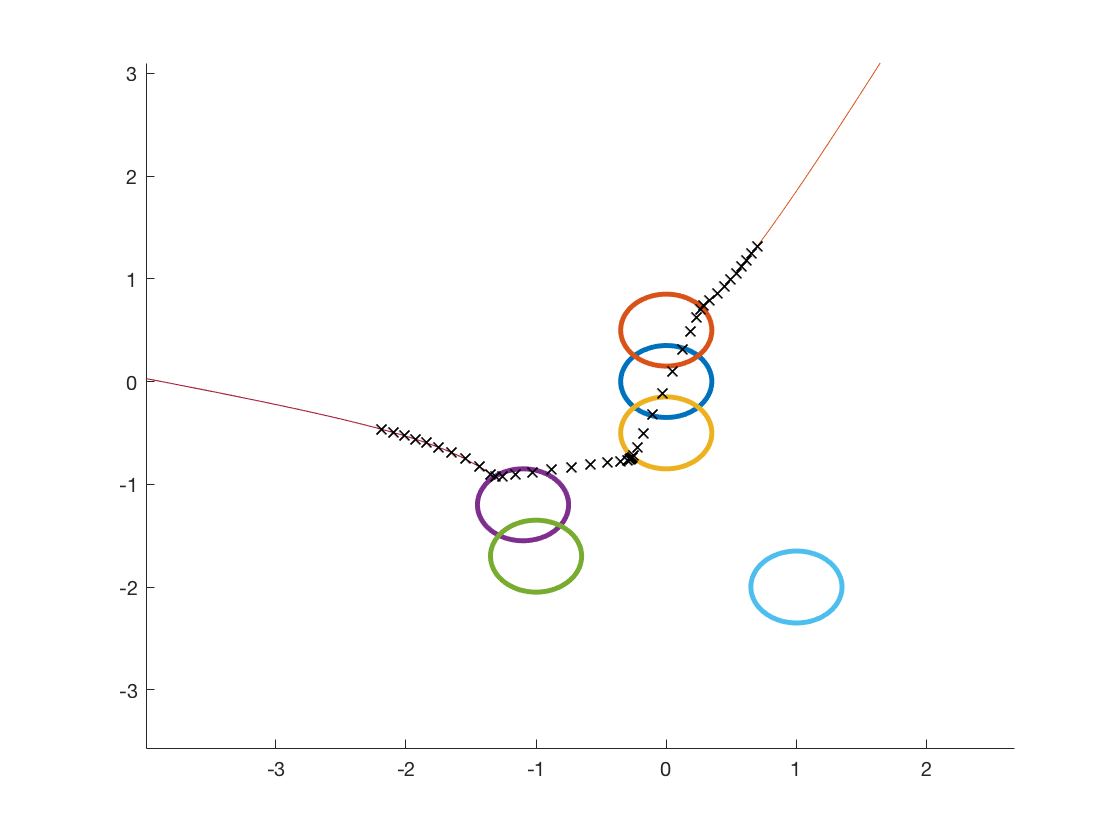
\includegraphics[width=0.7\linewidth]{../images/coalescEG}
		\caption{SD paths and nodes for \eqref{eq:meanPhase} in $\C$.}
		\label{fig:coalesceg}
	\end{figure}
	
	
	\section{Some results}
	
	Figure \ref{fig:chal1} shows plots of Challenge 1, for $250\times250$ Chebyshev nodes, which appear sufficient in the eyeball norm.
	
	Figure \ref{fig:chal2} shows some plots of Challenge 2, for $250\times250$ and $1000\times1000$ Chebyshev nodes respectively. In the eyeball norm it appears to be converging, although still not in total agreement with Dave's plot. There appear to be oscillations on a much finer scale than for Challenge 1. It should also be noted that the right-hand plot took around 12 hours to produce, so either more cores, more time, or a more sophisticated approach is necessary. 
		
		\begin{figure}[h]
		\centering
		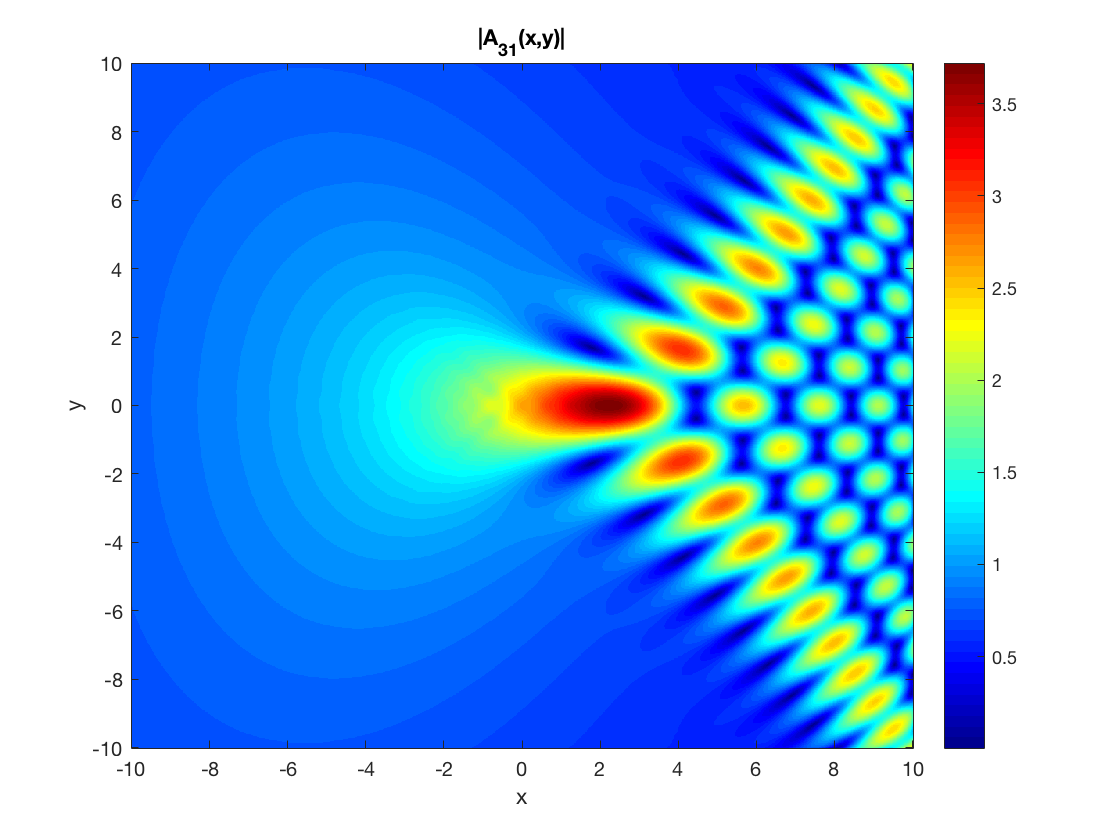
\includegraphics[width=0.45\linewidth]{../images/A31}
		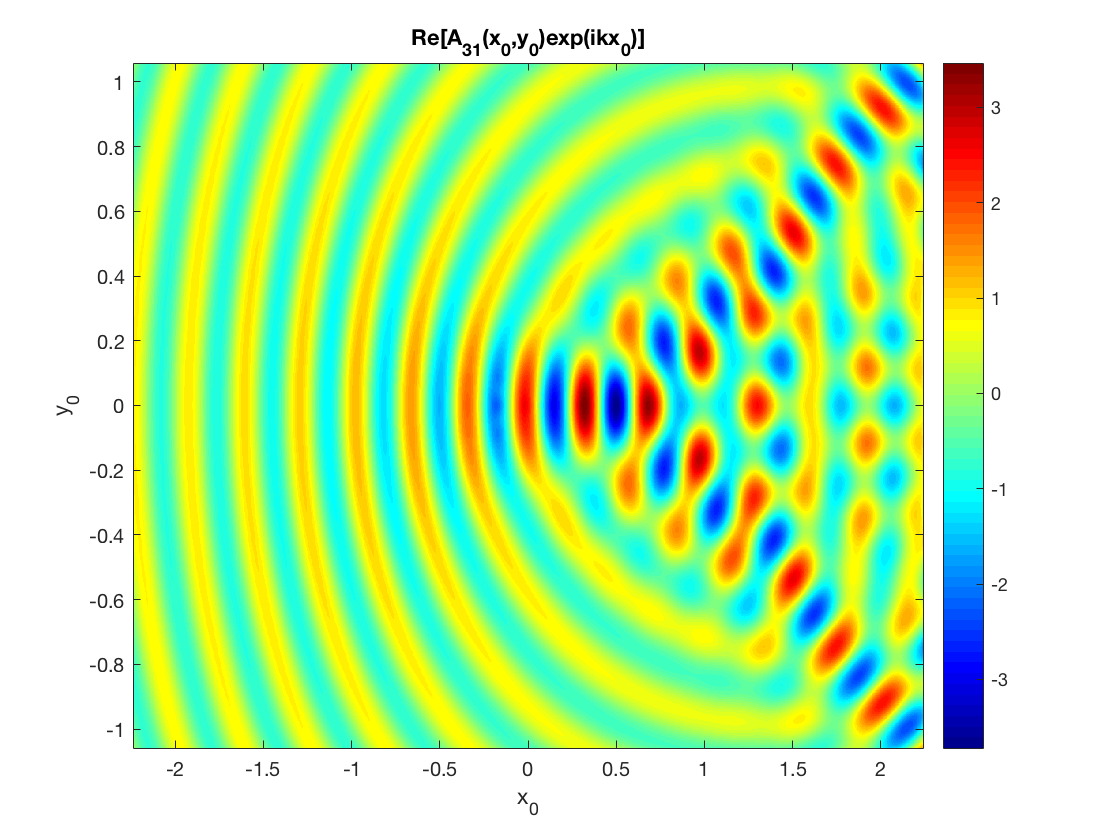
\includegraphics[width=0.45\linewidth]{../images/A31k20}
		\caption{Approximations of Challenge 1}
		\label{fig:chal1}
	\end{figure}
	
	\begin{figure}[h]
		\centering
		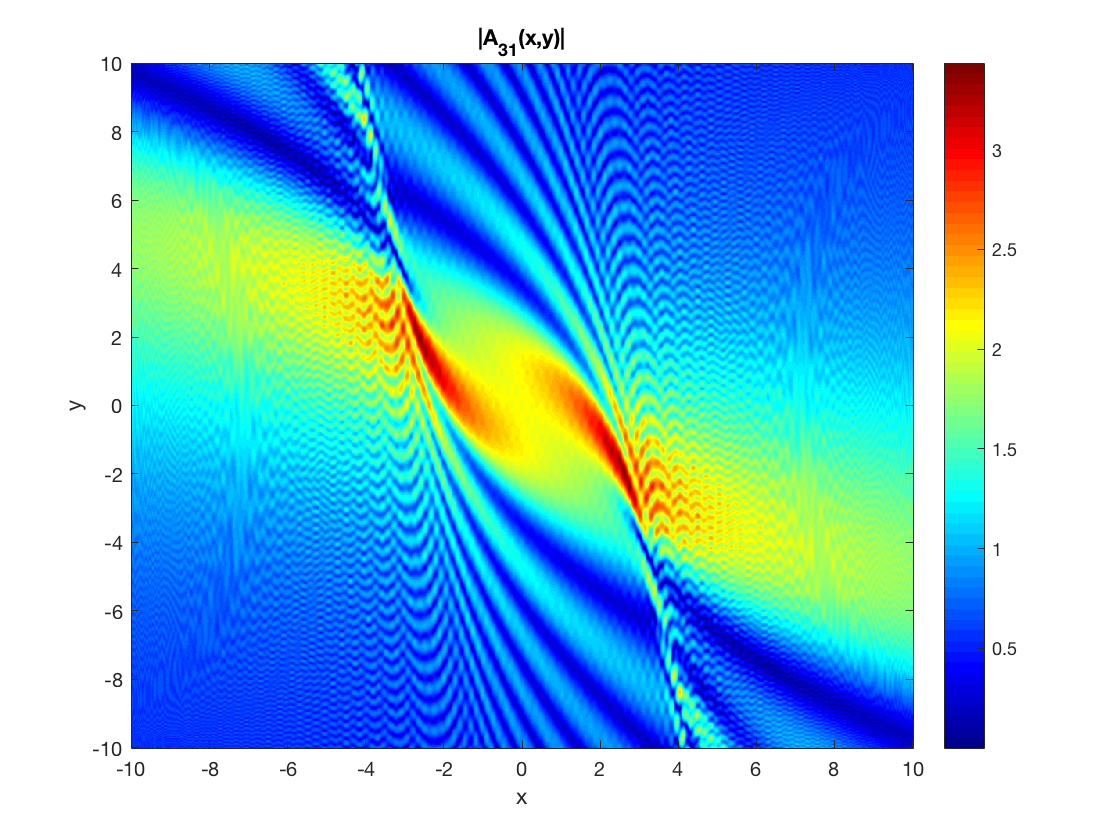
\includegraphics[width=0.45\linewidth]{../images/chal2_cheb250_quad_50}
		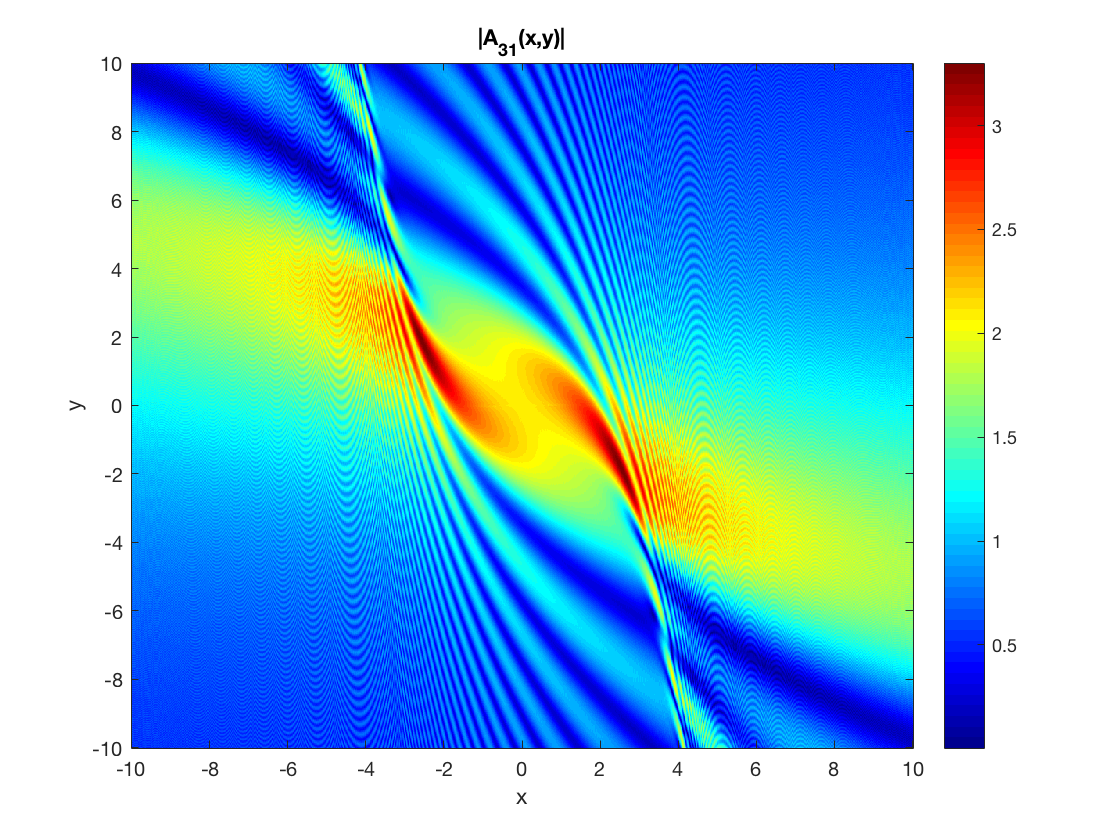
\includegraphics[width=0.45\linewidth]{../images/chal2_cheb1000_quad_50}
		\caption{Approximations of Challenge 2}
		\label{fig:chal2}
	\end{figure}

\section{A more sophisticated approach}

Each integral takes around 0.05s to approximate. This adds up when there are tens of thousands of integrals. A more sophisticated approach would involve partitioning the domain of interest (e.g. $[-10,10]^2$) into small subdomains, and a quadrature rule for the point at the centre of the domain is obtained. From here,
\begin{enumerate}
	\item This quadrature rule can be used for all other points in the domain, as the domain width and the perturbations in the phase $g$ are sufficiently small that we are still nearly on the path of steepest descent.
	\item This quadrature rule can be used as a starting point, which can then be iterated towards the path of steepest descent.
\end{enumerate}
	
	
	\begin{thebibliography}{9}
		\bibitem{DavePaper} 
		David P. Hewett, John R. Ockendon, Valery P. Smyshlyaev. 
		\textit{Contour integral solutions of the parabolic wave equation}. 
		arXiv:1806.02294v2, 2018.
	\end{thebibliography}

\end{document}